% !TEX root = ../my-thesis.tex
%
\chapter{Theoretical Foundations}
\label{sec:theory}
Before presenting the approach for tackling AutoML with an ensemble of optimizers, some theoretical foundations of both elements, AutoML and optimization, are given in the following.
This theoretical background is structured in three parts:
\begin{enumerate}
    \item Some basic concepts and intuitions of machine learning in general are outlined alongside with the challenges and problems that arise when applying machine learning.
    \item The concepts and usual approaches of AutoML are introduced, which were developed to tackle the listed challenges of classical machine learning. In addition, the connection between the AutoML setting and typical optimization problems is illustrated.
    \item As the foundation for building an ensemble of optimizers a selection of established optimization methods is given and explained.
\end{enumerate}
The overview of optimization methods is concluded with the discussion of a theoretical drawback of using a single optimization method.
This discussion of a possible disadvantage is used as a starting point for the line of reasoning why an ensemble of optimizers is an approach to counteract this drawback.
Before explaining the ensemble approach in the next chapter, this line of reasoning is continued with a selection of related works, where other approaches that addressed this theoretical disadvantage of using a single optimization method are mentioned. 

\section{Classical Machine Learning}
\label{sec:theory:ml}
If a human is given a task where the correct solution or reaction is not evident, a humans has always the possibility to react with a random solution or with an arbitrary reaction.
But if the human has any prior first- or second-hand experience with the same of a similar task, the human can choose the reaction based on the memories of different outcomes for different reactions for the more or less similar prior task.
With the high abstraction level and very symbolic nature of human thinking and memorization, it is comparably easy for humans to recognize even remote similarities between tasks.\newline
This is very challenging for a computer in contrast, because the models of tasks, experiences, and outcomes of reactions to tasks have to be readable and understandable for a machine, i.e. be in any kind of structured and consistent format.
This setting can be formalized as a combination of $T, P$ and $E$, where $T$ is a class of tasks, $P$ a performance measurement for solutions of a specific instances of the tasks class $T$ and $E$ is either given or collected experience, i.e. performance measurements for certain solutions in the context of specific task instance $t\in T$~\cite{Mitchell-MachineLearning}.\newline
Of course it is possible for a human programmer to manually specify the solution with the best performance measurement for any possible $t\in T$ but for a high $|T|$ this is rarely possible and viable.
Here, machine learning has its use-case: "Machine learning enables us to tackle tasks that are too difficult to solve with fixed programs written and designed by human beings"~\cite{Goodfellow-DeepLearning}.\newline
A high number of different types of task classes $T$ is imaginable, but one of the common one is \textit{Supervised Learning}.
In supervised learning, $T$ includes a fix set of all possible solutions $S$.
The concrete task for Supervised Learning is now to select for a given $t\in T$ a $s\subseteq S$ such that $P(t,s)$ is optimal.
To enable a machine to learn supervised, the experience $E$ has to be successively build in the form of $\{(t_1, s_1, P(t_1, s_1)), ..., (t_n, s_n, P(t_n s_n))\}$.
For a new task instance $t_i$, the computer will select a $s_i$ based on a decision model build from $E$, receive a performance feedback $P(t_i, s_i)$ and finally enrich $E$ with $(t_i, s_i, P(t_i, s_i))$ as well as updating the decision model with the changed $E$.
Therewith, a well working machine learning algorithm for supervised learning would now be able to achieve $P(t_j, s_j) \geq P(t_i, s_i)$ if $t_j$ and $t_i$ are similar instances, since it already has experience which $s\subseteq S$ had a certain performance value for $t_i$ and might therefore be a good or bad choice for $t_j$.\newline
This task of comparing and judging the similarity of different instances of $T$ and to build a practicable decision model based on $E$ to select a solution out of $S$ has been tackled with a plethora of different algorithms or even combinations of multiple algorithms as a form of machine learning pipeline.
Usually, this algorithms have to be configured with a set of hyperparameter depending on $T$ and often $T$ also has to be transformed before presenting concrete instances to the algorithm for learning, i.e. pre-processing each $t\in T$ with one or more transformation methods.
Without making suitable choices for the machine learning algorithm as well as corresponding hyperparameter and pre-processing methods for each different $T$, the performance measurements will only increase for a high $|E|$ or even not at all.
But because the number of available task instances, i.e. the amount of data, that can be used to build $E$ with a machine learning algorithm is often limited for most use-case domains, a valid choice for the learning algorithm, hyperparameter and, if necessary, pre-processing methods is crucial.\newline
With the high number of available machine learning algorithms and the often complex relationships between learning performance and hyperparameter configurations of the chosen algorithm as well as properties of $T$ and suitable pre-processing methods a big expertise in the machine learning field is necessary to be able to assemble machine learning applications with good performance measurements.
Since this necessary expertise in machine learning is not broadly available and a lot of companies or research facilities have a high demand for machine learning applications, it is not possible to apply machine learning in every use-case where it might be beneficial.
This accelerated the emergence of the machine learning research sub-topic \textit{Automated Machine Learning}. 

\section{Automated Machine Learning}
\label{sec:theory:automl}
Automated Machine Learning, or short \textit{AutoML}, tries to tackle this knowledge barrier, which prevents interested people from applying machine learning.
Therefore, the overall goal is to automate most tasks of the process of creating a machine learning application that would require machine learning knowledge.\newline
In this chapter at first a description of the general workflow of an AutoML tool is given and the usual two main steps of this workflow are illustrated.
This will be concluded with an formalization of the AutoML problem setting as an optimization problem.

\subsection{General Workflow}
\label{sec:theory:automl:workflow}
AutoML application are usually designed very homogeneous and therefore have very similar workflows among themselves.
As an input, the application will receive data in an machine-readable format and usually some form of constraint for its execution.
The expected outputs are the performance of the found machine learning pipeline regarding some task-dependent metric and the best found machine learning pipeline for the given data itself.
Additionally, each AutoML tool can have further configuration necessary as an input.\newline
The constraints for execution are required to prevent the AutoML tool from searching for the best machine learning pipeline for the given data indefinitely with probably continuously growing hardware consumption.
Therefore, the time and/or some hardware budgets are constrained.
This inputs and outputs of an conceptual AutoML tool are illustrated in figure~\ref{fig:theory:conceptualAutoMLTool}.\newline
\begin{figure}
    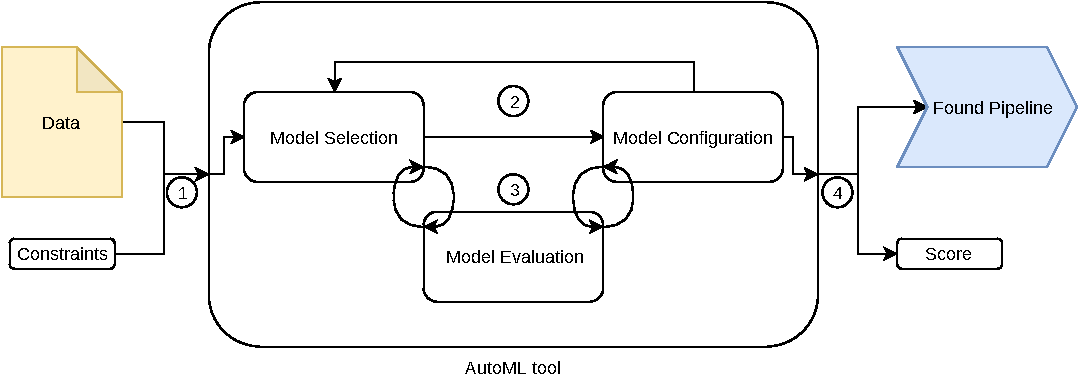
\includegraphics[width=\textwidth]{gfx/Figures/AutoMLTool.pdf}
    \caption{High level view of a conceptual AutoML tool. }
	\label{fig:theory:conceptualAutoMLTool}
\end{figure}
The general workflow of an AutoML tool is also numbered and illustrated in the figure and can be generalized with the following steps:
\begin{enumerate}
    \item AutoML tool gets input data and some execution constraints as an input.
    \item Model Selection and Model Configuration are repeated until execution constraints are met.
    \item Model Selection as well as Model Configuration can perform a Model Evaluation to get a score for any pipeline candidate they encounter.
    \item After the constraints are met, the best found pipeline as well as the score of this pipeline are given as an output.
\end{enumerate}
The Model Evaluation step is usually performed by training a pipeline on one big portion of the input data and testing it with a smaller portion of the data while measuring some kind of performance measurement, for example the accuracy of predictions or some error metric.
But other evaluation techniques for example like a Cross-Validation are also common.\newline
While the Model Evaluation step is only very loosely defined and usually not a complex procedure, the Model Selection and Model Configuration steps of the AutoML workflow are more sophisticated and will be individually explained in the following.

\subsection{Model Selection}
\label{sec:theory:automl:selection}
Model Selection is the task of selecting $1$ to $n$ components that will be part of the machine learning pipeline and sequentially traversed when data is passed through the pipeline.
For example, a valid pipeline would be to apply a Principal-Component-Analysis on the data as a first component and to use a Support Vector Machine for classification on the processed data as a second component afterwards.\newline
Usually there are three types of components:
\begin{itemize}
    \item Pre-Processing: Transform the input data before presenting it to the learning model.
    \item Learning Model: Perform the actual machine learning task on the data, for example classify a datapoint after training.
    \item Post-Processing: Transform the output of the learning model before yielding it as a final result.
\end{itemize}
Although in theory only a single learning model is necessary and components for pre- and post-processing are optional, at least pre-processing is very common in machine learning pipelines and included most of the time.\newline
It is possible to use more than one component from each type in a single pipeline and pipelines with arbitrary complexity can be created.
More than one pre- or post-processor can be used in sequence or in parallel with some kind of aggregator subsequently.
Equally, more than one learning model can be combined to be used as a composite model with a proper aggregation method like for example Bagging of models~\cite{Breiman-BaggingPredictors}.
An example for such a complex pipeline is illustrated in figure~\ref{fig:theory:complexPipeline}\newline
\begin{figure}
    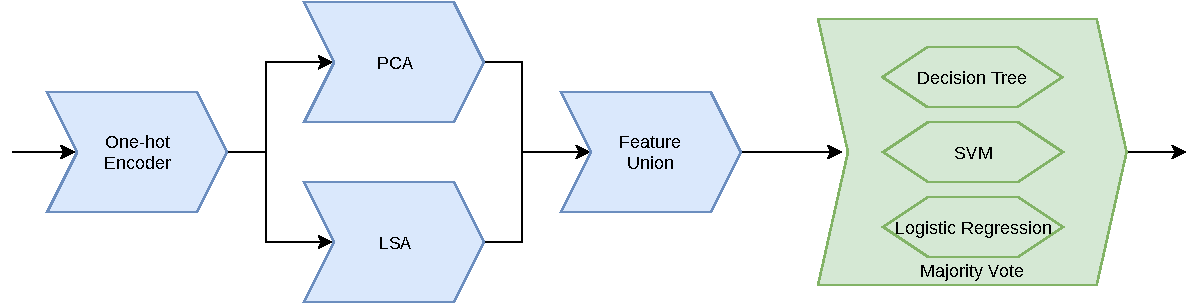
\includegraphics[width=\textwidth]{gfx/Figures/ComplexPipeline.pdf}
    \caption{Example for a more complex pipeline with four pre-processing components in blue: A One-hot Encoder, a Feature Union of a PCA and a LSA. The learning model in green is a Majority Voter as an aggregation of a Decision Tree, a SVM and a Logistic Regression Classifier. }
	\label{fig:theory:complexPipeline}
\end{figure}
Model Selection where the resulting pipelines can have this complexity needs to add a structural relationship between the pipeline components to the selected components.
Therewith, Model Selection can be written as simple formalization with two things:
\begin{itemize}
    \item For all possible components $C=\{c_1, ..., c_n\}$ a $C' \subseteq C$ of components that will be used to construct the pipeline.
    \item A binary relation $\prec$ over $C'$ that defines which component is a data input for another component to define an order of the components for the pipeline as well as aggregation of several components with one component. 
\end{itemize}
Nevertheless, to find a valid set $C' \subseteq C$ is not a trivial task.
For example, when a aggregator for multiple parallel pre-processing components is needed a valid choice could be a Feature Union component but a Decision Tree component would be invalid for this pipeline position.
Therefore, if the pipelines shall be allowed to be more complex than for example a single pre-processing component and a single learning model, there is a big set of constraints for valid subsets of $C$.

\subsection{Model Configuration}
\label{sec:theory:automl:configuration}
With the resulting component set of a Model Selection step $C'=\{c_1, ..., c_r\}$ the pipeline is not ready to be used yet, because usually each component has a set of hyperparameter and for each one a concrete value is needed.
Each component $c_k$ has a set of hyperparameter $\Theta_k=\{ \theta_{k,1}, ..., \theta_{k,j} \}$ where each hyperparameter has a range where the value for this hyperparameter has to be chosen from.
Such a range can for example be a numeric set $\mathbb{N}$ or a custom set like for example $\{\textrm{true}, \textrm{false}\}$.\newline
When combining all ranges $\bigcup\limits_{i=1}^r \Theta_i$ a parametrization space with dimension $r$ is defined, where configuration vectors can be drawn from to configure a pipeline instance created from $C'$.
An example for a concrete parametrization drawn from a three dimensional parameter space is shown in figure~\ref{fig:theory:parameterSpace}
\begin{figure}
    \begin{tikzpicture}
        \begin{axis}[
          view={35}{15},
          axis lines=center,
          width=15cm,height=15cm,
          xtick={0.25, 0.5, 0.75},ytick={5,10, 15},ztick={-10,-5,5,10},
          xmin=0,xmax=1,ymin=0,ymax=20,zmin=0.5,zmax=2.5,
          zticklabels={true, false},ztick={1,2},
          z tick label style={anchor=east}]
        ]
        \addplot3 [only marks] coordinates {(0.4,10,1)};
        \addplot3 [no marks,densely dashed] coordinates { (0.4,0,0.5) (0.4,10,0.5) (0.4,10,1)};
        \node [above right] at (axis cs:0.4,10,1) {$(0.4,10,\textrm{true})$};
        \end{axis}
    \end{tikzpicture}
    \caption{A parameter configuration with the values $(0.4,10,\textrm{true})$ inside the parameter space with the dimensions $[0..20]$, $[0, 1)$ and $\{\textrm{true}, \textrm{false}\}$ }
	\label{fig:theory:parameterSpace}
\end{figure}
When such a vector is drawn a concrete pipeline from all selected components can be constructed and configured with the vector values to be evaluated as a candidate pipeline.

\subsection{Formalization of AutoML as an Optimization Problem}
\label{sec:theory:automl:optimization}

\Blindtext


\section{Black Box Optimization}
\label{sec:theory:optimization}

\Blindtext

\subsection{Differences to General Optimization Problems}
\label{sec:theory:optimization:differences}

\Blindtext

\subsection{Optimization by Searching}
\label{sec:theory:optimization:search}

\Blindtext

\subsection{Genetic and Evolutionary Optimization}
\label{sec:theory:optimization:genetic}

\Blindtext

\subsection{Bayesian Optimization}
\label{sec:theory:optimization:bayesian}

\Blindtext

\subsection{No-Free-Lunch Theorem}
\label{sec:theory:optimization:lunch}

\Blindtext

\section{Related Work}
\label{sec:theory:related}

\Blindtext
